\section{Einleitung und Versuchsziel}
\label{sec:aufgabenstellung}
%In der Aufgabenstellung wird (in eigenen Worten und ganzen Sätzen) formuliert, was das Ziel des 
%Versuches ist.  
%[Beachten Sie die eigentliche Aufgabenstellung in den Versuchsanleitungen sowie die Hinweise zur Auswertung!] 

Im folgenden Versuch werden die Grundlagen des Wärmepumpenprozesses an einer Beispielanlage untersucht und die Ergebnisse verschiedener Fahrweisen diskutiert. Es werden Kenntnisse zu linksläufigen Kreisprozessen, Arbeit mit einem $\lg{p}, h$-Diagramm, sowie die energetische Bilanzierung der einzelnen Apparate und des Gesamtprozesses.
In den folgenden Abbildungen \ref{fig:schema1}, \ref{fig:schema2} und \ref{fig:tech_zeichnung} sind zwei schematische Skizzen, sowie der technische Versuchsaufbau der zwei grundlegenden Fahrweisen dargestellt.

\begin{figure}[h!]
	\centering
	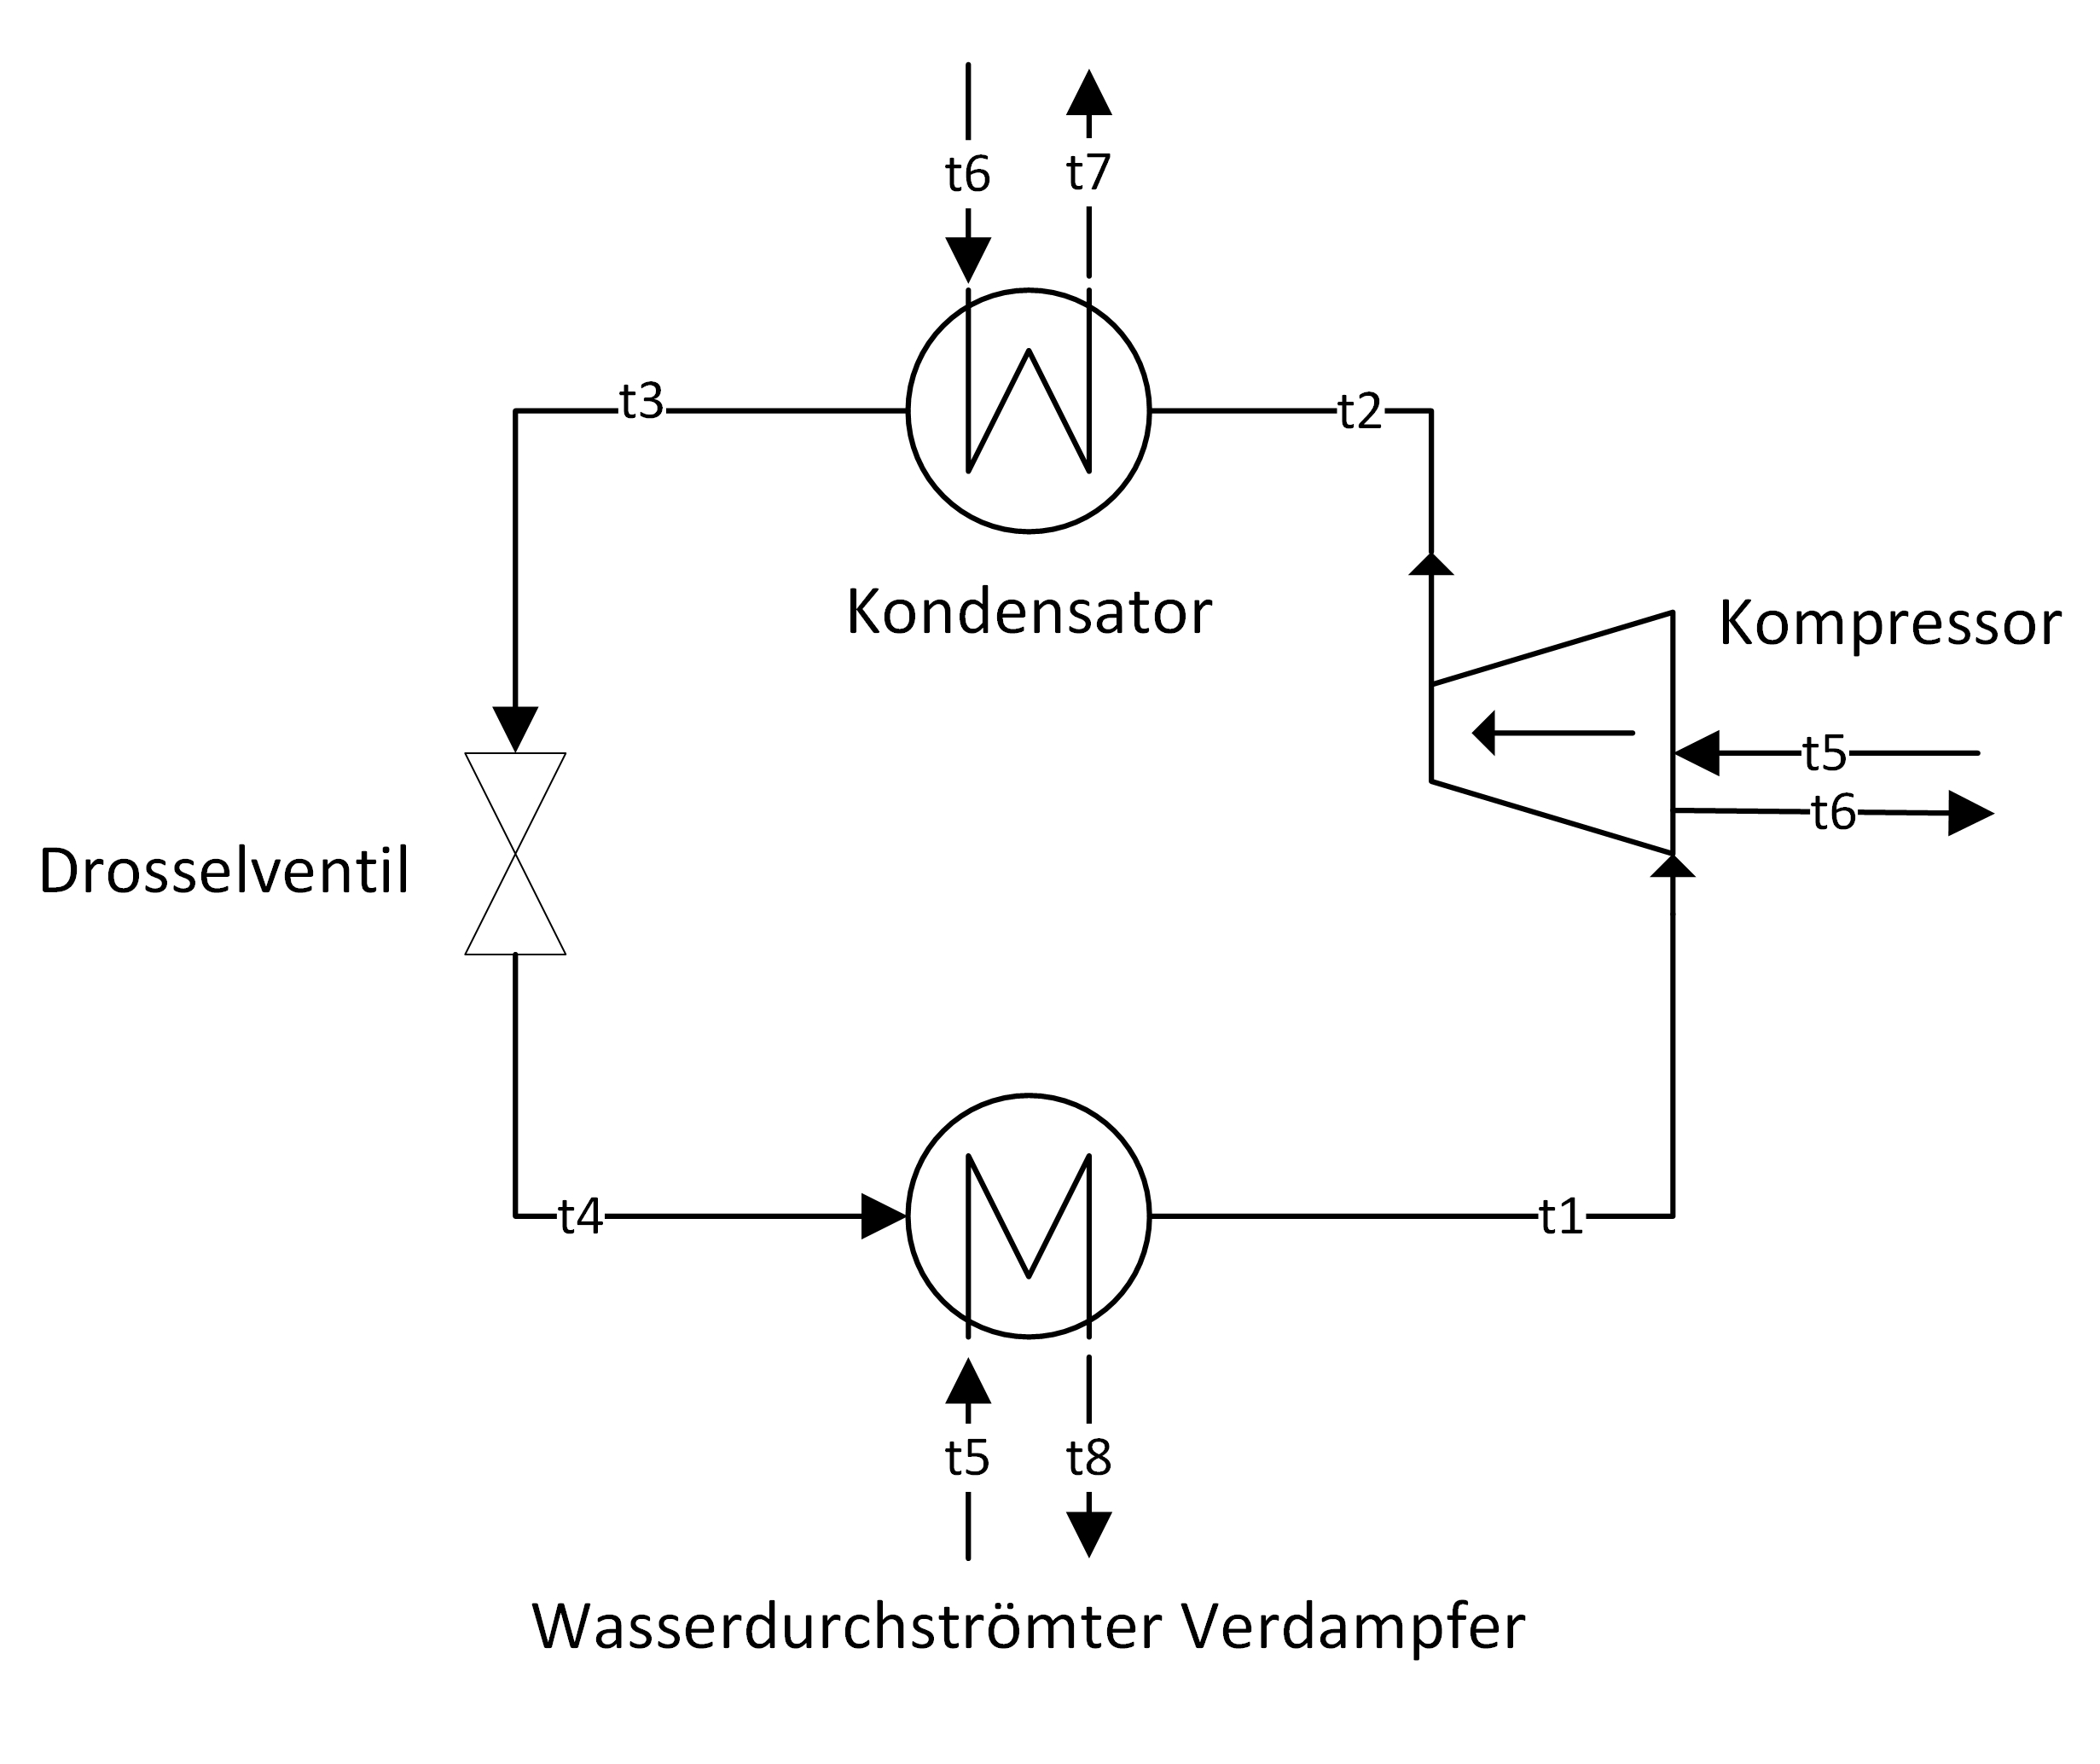
\includegraphics[width=0.5\textwidth]{img/schema2}
	\caption{Schematik des Versuchsaufbaus mit wasserdurchströmten Verdampfer}
	\label{fig:schema1}
\end{figure}
\FloatBarrier

\begin{figure}[h!]
	\centering
	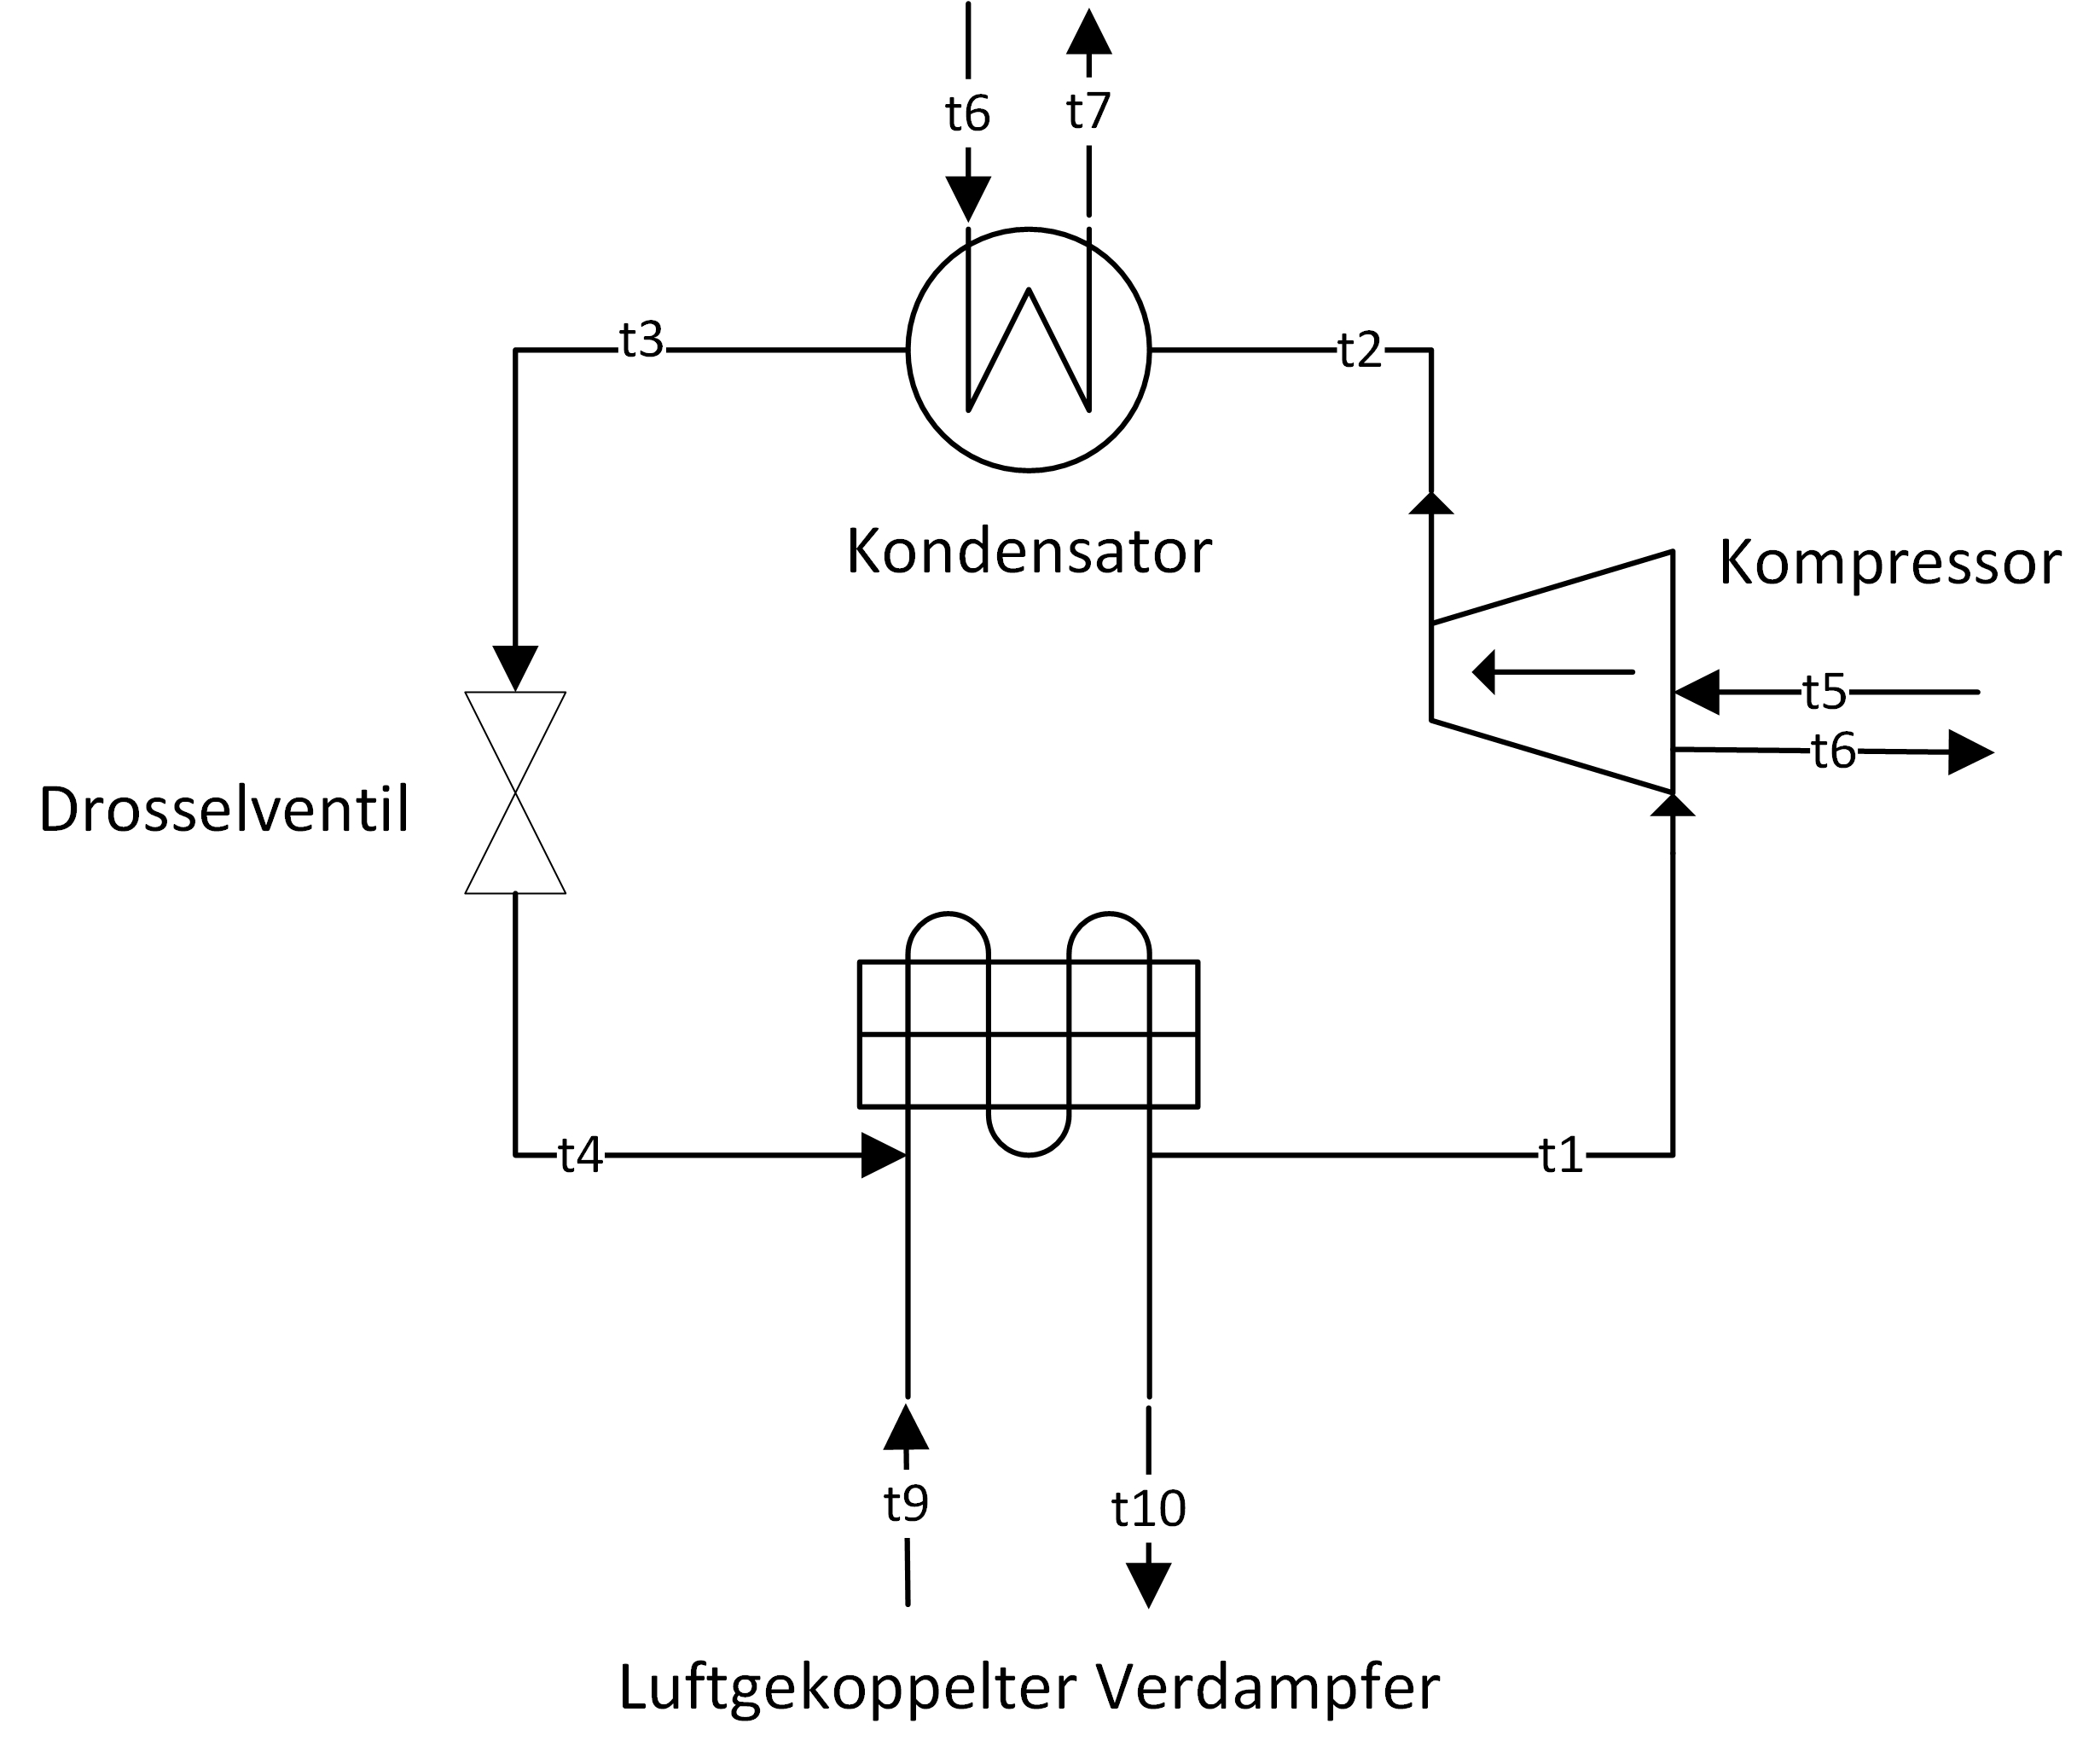
\includegraphics[width=0.5\textwidth]{img/schema1}
	\caption{Schematik des Versuchsaufbaus mit luftgekoppelten Verdampfer}
	\label{fig:schema2}
\end{figure}
\FloatBarrier

\begin{figure}[h!]
	\centering
	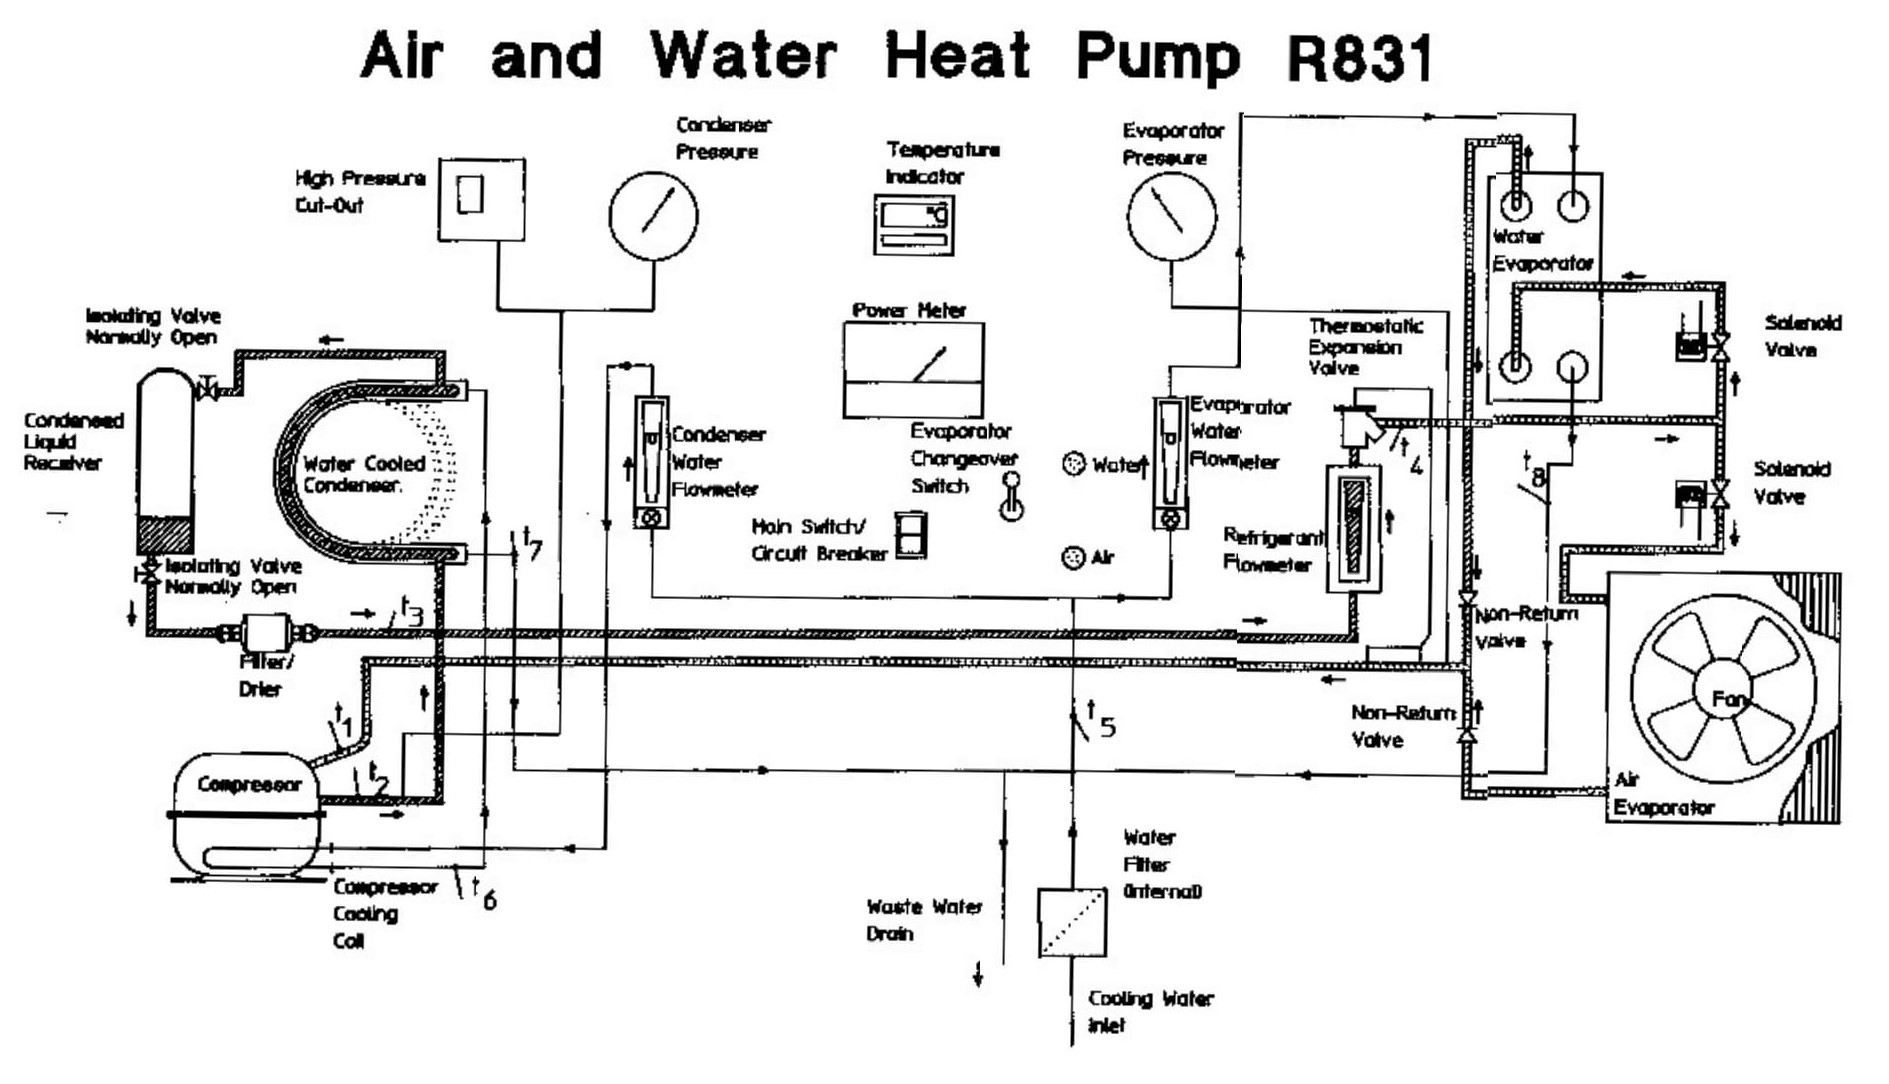
\includegraphics[width=1.0\textwidth]{img/zeichnung-1}
	\caption{Technische Zeichnung des Versuchsaufbaus}
	\label{fig:tech_zeichnung}
\end{figure}
\FloatBarrier


